\documentclass[border=4pt]{standalone}
% Shared typography and colours for the standalone figures.
\usepackage{unicode-math}
\setmainfont{TeX Gyre Termes}
\setmathfont{TeX Gyre Termes Math}
\usepackage{tikz}
\usetikzlibrary{arrows.meta,positioning,calc,decorations.pathreplacing}
\usepackage{pgfplots}
\pgfplotsset{compat=1.18}
\definecolor{elemA}{HTML}{1F5FA8}
\definecolor{elemB}{HTML}{B8461B}
\definecolor{elemC}{HTML}{2E7D32}
\definecolor{elemD}{HTML}{6A4C93}
\definecolor{frameline}{HTML}{555555}

\begin{document}
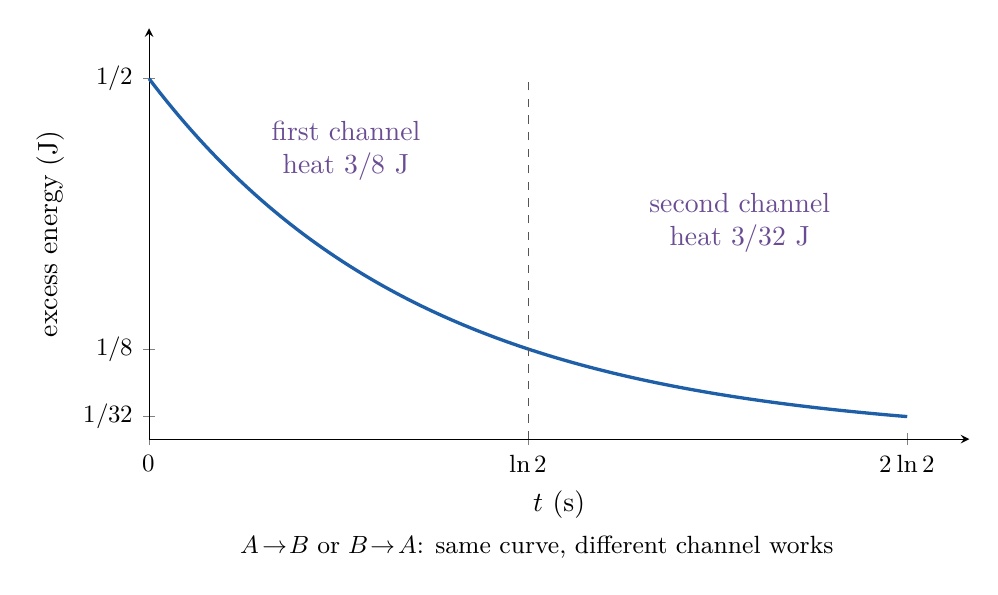
\begin{tikzpicture}
\begin{axis}[width=12cm,height=6.8cm,xmin=0,xmax=1.5,ymin=0,ymax=.57,
 axis lines=left,xlabel={$t$ (s)},ylabel={excess energy (J)},
 xtick={0,.69314718056,1.38629436112},xticklabels={$0$,$\ln2$,$2\ln2$},
 ytick={.03125,.125,.5},yticklabels={$1/32$,$1/8$,$1/2$},
 tick label style={font=\small},clip=false]
\addplot[elemA,very thick,domain=0:1.38629436112,samples=151] {.5*exp(-2*x)};
\draw[dashed,frameline] (axis cs:.69314718056,0)--(axis cs:.69314718056,.5);
\node[align=center,elemD] at (axis cs:.36,.4) {first channel\\heat $3/8$ J};
\node[align=center,elemD] at (axis cs:1.08,.3) {second channel\\heat $3/32$ J};
\node[anchor=north west,font=\small] at (axis cs:.15,-.12)
 {$A\!\to\!B$ or $B\!\to\!A$: same curve, different channel works};
\end{axis}
\end{tikzpicture}
\end{document}
